%\documentclass[12pt]{article}

\questionheader{ex:s1.2}

%%%%%%%%%%%%%%%%%%
\subsection*{\Conceptual}
%%%%%%%%%%%%%%%%%%

\begin{question}
A curve $\vr(s)$ is parametrized in terms of arclength. What is  $\displaystyle\int_1^t |\vr'(s)|\,\dee{s}$ when $t \ge 1$?
\end{question}
\begin{hint}
You're asked to find the arclength of the curve from $s=1$ to $s=t$.
\end{hint}
\begin{answer}
$t-1$
\end{answer}
\begin{solution}
By Lemma \eref{CLP317}{lem:CVtanArclen}.c in the CLP-4 text, $|\vr'(s)|=1$
under arclength parametrization. So 
$\int_1^t |\vr'(s)|\dee{s}=\int_1^t \dee{s}=t-1$.
\end{solution}
%%%%%%%%%%%%%%%%%%



\begin{question}
The function
\[\vr(s)=\sin\left(\frac{s+1}{2}\right)\hi+\cos\left(\frac{s+1}{2}\right)\hj+\frac{\sqrt3}{2}(s+1)\hk\]
 is parametrized in terms of arclength, starting from the point $P$. What is $P$?
\end{question}
\begin{hint}
The arclength will be 0 at $P$.
\end{hint}
\begin{answer}
$\left( \sin(1/2),\cos(1/2),\sqrt{3}/2\right)$
\end{answer}
\begin{solution}
The arclength from $P$ to $P$ will be 0, so $P$ is the point where $s=0$. That is, $\vr(0)$, or 
$\left( \sin(1/2),\cos(1/2),\sqrt{3}/2\right)$.
\end{solution}
%%%%%%%%%%%%%%%%%%

\begin{question}
A curve $\vR=\va(t)$ is reparametrized in terms of arclength as $\vR=\vb(s)=\va(t(s))$. Of the following options, which best describes the relationship between the vectors $\va'(t_0)$ and $\vb'(s_0)$, where $t(s_0)=t_0$?

You may assume $\va'(t)$  and $\vb'(s)$ exist and are nonzero for all $t,s\ge0$.
\begin{enumerate}[A.]
\item they are parallel and point in the same direction
\item they are parallel and point in opposite directions
\item they are perpendicular
\item they have the same magnitude
\item they are equal
\end{enumerate}
\end{question}
\begin{hint}
$\va(t_0)$ and $\vb(s_0)$ describe the same point on $\vR$.
\end{hint}
\begin{answer}
A
\end{answer}
\begin{solution}
\begin{description}
\item[\textbf{Solution 1:}]
We consider the situation geometrically. If we plot $\vR$ in space (of the relevant dimension), regardless of its parametrization, the derivative at a point will give a vector tangent to $\vR$, in the direction the curve moves when the parameter is increasing. Since $\va(t_0)$ and $\vb(s_0)$ describe the same spot on the curve, $\va'(t_0)$ and $\vb'(s_0)$ will be parallel\footnote{Since we specified the derivatives are nonzero, there's no messiness about vectors being parallel to a zero vector.} --- they're both tangent to the same piece of curve. Furthermore, as $t$ increases, so does $s$, so the direction of increasing $t$ is the same as the direction of increasing $s$. Therefore, A. holds.
\begin{center}
\begin{tikzpicture}
\draw[thick] plot[domain=-1:1.75]({\x*\x*\x-\x*\x},\x);
\draw (-2,-1) node[below]{$\vR$};
\draw (25/64,1.25) node[vertex, label=below right:{$\va(t_0)=\vb(s_0)$}]{};
\draw[thick, blue] plot[domain=-2:2.5] (\x,{0.457*(\x-25/64)+1.25})node[right]{tangent direction};
\end{tikzpicture}
\end{center}
Now we consider the magnitudes of the vectors, to rule out E. Recall $|\va'(t)|$ is the speed at which the curve changes relative to $t$; this could be any (nonnegative) number. By the same token, $ |\vb'(s)|=1$. So, $\vb'(s_0)$ is a unit vector, while $\va'(t_0)$ may or may not be. Then the two vectors are not \emph{necessarily} equal (although they could be).

So, the best answer is A. 
\item[\textbf{Solution 2:}] The chain rule gives us a relationship between $\vb'(s)$ and $\va'(t)$.
\begin{align*}
\diff{\vb}{s}&=\diff{}{s}[\va(t(s))]=\diff{\va}{t}\,\diff{t}{s}
\end{align*}
So, the vectors $\diff{\vb}{s}$ and $\diff{\va}{t}$ differ only by the scalar function $\diff{t}{s}$. So, at any point along the curve, these vectors are parallel.

Furthermore, we know that $t$ and $s$ are positively correlated: as $t$ increases, so does $s$, because we're covering more arclength. So, $\diff{t}{s}$ is nonnegative. Furthermore, since the derivatives are nonzero, $\diff{t}{s}$ is nonzero. So, $\vb'(s_0)$ and $\va'(t_0)$ are positive scalar multiples of each other. That is, they are parallel, and pointing in the same direction. However, unless $\diff{t}{s}=1$ (that is, $t(s)=s+C$ for some constant $C$), the vectors do not have the same magnitude, and hence are not equal.

So, A is the best solution. 
\end{description}
\end{solution}
%%%%%%%%%%%%%%%%%%

%%%%%%%%%%%%%%%%%%
\subsection*{\Procedural}
%%%%%%%%%%%%%%%%%%


\begin{question}[M317 2012D] %2

\begin{enumerate}[(a)]
\item
Let
\begin{equation*}
\vr(t) = (2 \sin^3 t , 2\cos^3 t, 3 \sin t \cos t)
\end{equation*}
Find the unit tangent vector to this parametrized curve at $t = \pi/3$, 
pointing in the direction of increasing $t$.
\item
Reparametrize the vector function $\vr(t)$ from (a) with respect to 
arc length measured from the point $t = 0$ in the direction of increasing $t$.
\end{enumerate}
\end{question}

\begin{hint} 
On your way to finding the relationship between $t$ and arclength, you should realize that the curve has constant speed (with respect to $t$), though not constant velocity.
\end{hint}

\begin{answer} 
(a) $\big(\nicefrac{3}{4}\,,\,
                -\nicefrac{\sqrt{3}}{4}\,,\,-\nicefrac{1}{2}\big)$\qquad
(b) $\vR(s) = \big(2 \sin^3(\nicefrac{s}{3}) , 2\cos^3(\nicefrac{s}{3}), 
       3 \sin(\nicefrac{s}{3}) \cos(\nicefrac{s}{3})\big)$
\end{answer}

\begin{solution} (a) The velocity vector is
\begin{align*}
\vr'(t) &= (6\sin^2(t)\cos t\,,\, -6\sin t\cos^2(t)\,,\, 3\cos^2t-3\sin^2t) \\
        &= 3\big(\sin t \sin(2t)\,,\,-\cos t\sin(2t)\,,\,\cos(2t)\big)
\end{align*}
In particular, since $\sin(\pi/3)=\sin(2\pi/3)=\frac{\sqrt{3}}{2}$
and $\cos(\pi/3)=-\cos(2\pi/3)=\frac{1}{2}$,
\begin{align*}
\vr'(\pi/3)  &= 3\big(\nicefrac{3}{4}\,,\,
                -\nicefrac{\sqrt{3}}{4}\,,\,-\nicefrac{1}{2}\big)
\end{align*}
and the specified unit tangent vector is
\begin{align*}
\hat\vT &= \frac{\big(\nicefrac{3}{4}\,,\,
                -\nicefrac{\sqrt{3}}{4}\,,\,-\nicefrac{1}{2}\big)}
               {\big|\big(\nicefrac{3}{4}\,,\,
                -\nicefrac{\sqrt{3}}{4}\,,\,-\nicefrac{1}{2}\big)\big|} 
        =\big(\nicefrac{3}{4}\,,\,
                -\nicefrac{\sqrt{3}}{4}\,,\,-\nicefrac{1}{2}\big)
\end{align*}

\noindent (b)
The speed is
\begin{align*}
\diff{s}{t} 
  &= |\vr'(t)| = 3\sqrt{\sin^2t\sin^2(2t)+\cos^2t\sin^2(2t)+\cos^2(2t)} \\
  &= 3\sqrt{\sin^2(2t)+\cos^2(2t)} \\
  &=3
\end{align*}
So $s=3t$ and the reparametrized form is
\begin{align*}
\vR(s) = \big(2 \sin^3(\nicefrac{s}{3}) , 2\cos^3(\nicefrac{s}{3}), 
       3 \sin(\nicefrac{s}{3}) \cos(\nicefrac{s}{3})\big)
\end{align*}

\end{solution}
%%%%%%%%%%%%%%%%%%%%%%%%%%%



%%%%%%%%%%%%%%%%%%%%%%%%%%%
\begin{question}[M317 2008D]\label{prob_s1.2:spiral} %1
This problem is about the logarithmic spiral in the plane
\begin{equation*}
\vr(t) = e^t (\cos t, \sin t),\qquad t \in \bbbr
\end{equation*}
\begin{enumerate}[(a)]
\item
Find the arc length of the piece of this spiral which is contained in the unit
circle.
\item
Reparametrize the logarithmic spiral with respect to arc length, measured
from $t = -\infty$.
\end{enumerate}
\end{question}

\begin{hint} 
For which values of $t$ is $|\vr(t)|\le 1$? Check the domain of $t$ --- we're not starting at zero.
\end{hint}

\begin{answer} 
(a) $\sqrt{2}$\qquad
(b) $\frac{s}{\sqrt{2}}\left(\cos\Big(\ln\Big(\frac{s}{\sqrt{2}}\Big)\Big)\,,\,
                 \sin\Big(\ln\Big(\frac{s}{\sqrt{2}}\Big)\Big)\right)$
\quad\text{with $s>0$}
\end{answer}

\begin{solution} (a) We have $|\vr(t)|=e^t\le 1$ for $t\le 0$.
So the part of the spiral contained in the unit circle is the part of 
the spiral with $-\infty<t\le 0$.
As
\begin{align*}
\vr'(t) = e^t (\cos t, \sin t) + e^t (-\sin t, \cos t)
        =e^t\big(\cos t -\sin t\,,\,\sin t + \cos t\big)
\end{align*}
the speed
\begin{align*}
\diff{s}{t} = \big|\vr'(t)\big|
            = e^t \sqrt{(\cos t-\sin t)^2+(\sin t+\cos t)^2}
            = \sqrt{2}e^t
\end{align*}
and the arclength from $t=-\infty$ to $\vr(t)$ is
\begin{equation*}
s(t)=\int_{-\infty}^t \diff{s}{t}(\tilde t)\ \dee{\tilde t}
    =\int_{-\infty}^t \sqrt{2} e^{\tilde t}\ \dee{\tilde t}
    =\sqrt{2}e^t
\end{equation*}
In particular the length of the part of the spiral contained in the
unit circle is $s(0)=\sqrt{2}$.

\noindent (b)
The inverse function of $s(t)=\sqrt{2} e^t$ is
$t(s) =\ln\left(\frac{s}{\sqrt{2}}\right)$ with $s>0$. 
(As $t\rightarrow-\infty$, the arc length $s\rightarrow 0$ and 
as $t\rightarrow+\infty$, the arc length $s\rightarrow +\infty$.)
So the reparametrization is
\begin{align*}
\vR(s) = e^t (\cos t, \sin t)\Big|_{t=\ln\left(\frac{s}{\sqrt{2}}\right)}
=\frac{s}{\sqrt{2}}\left(\cos\Big(\ln\Big(\frac{s}{\sqrt{2}}\Big)\Big)\,,\,
                 \sin\Big(\ln\Big(\frac{s}{\sqrt{2}}\Big)\Big)\right)
\quad\text{with $s>0$}
\end{align*}


\end{solution}


%%%%%%%%%%%%%%%%%%%%%%%%%%%%
%%%very similar to [M317 2012D] %2 --- equation is off by a constant, other question has an (a) and (b) part
%\begin{question}[M317 2006D] %5
%Let
%\begin{align*}
%\vr(t) = \cos^3t\,\hi + \sin^3t\,\hj + \frac{3}{2}\sin t \cos t\,\hk
%\end{align*}
%Reparameterize $\vr(t)$ with respect to arclength measured from 
%the point $t = 0$ in the direction of increasing $t$.
%\end{question}

%\begin{hint} 
%
%\end{hint}

%\begin{answer} 
%$\cos^3\frac{2s}{3}\,\hi + \sin^3\frac{2s}{3}\,\hj 
%             + \frac{3}{2}\sin \frac{2s}{3} \cos \frac{2s}{3}\,\hk$
%\end{answer}

%\begin{solution}
%The velocity is
%\begin{align*}
%\vr'(t) &= -3\cos^2t\sin t\,\hi + 3\sin^2t\cos t\,\hj 
%         + \frac{3}{2}\big[\cos^2 t -\sin^2 t\big]\,\hk \\
%        &= -\frac{3}{2}\cos t \sin(2t)\,\hi +\frac{3}{2}\sin t\sin(2t)
%           +\frac{3}{2}\cos(2t)\,\hk
%\end{align*}
%so that speed is
%\begin{align*}
%\diff{s}{t} & = \frac{3}{2}\sqrt{\cos^2t \sin^2(2t) 
%                                +\sin^2t \sin^2(2t)
%                                 +\cos^2(2t)} 
%               =\frac{3}{2}
%\end{align*}
%So $s=\frac{3}{2}t$ and $t=\frac{2s}{3}$ and the reparametrization is
%\begin{align*}
%\cos^3\frac{2s}{3}\,\hi + \sin^3\frac{2s}{3}\,\hj 
%             + \frac{3}{2}\sin \frac{2s}{3} \cos \frac{2s}{3}\,\hk
%\end{align*}

%\end{solution}


%%%%%%%%%%%%%%%%%%
\subsection*{\Application}
%%%%%%%%%%%%%%%%%%

\begin{question}
Define
\[\vr(t)=\left(\frac{1}{\sqrt{1+t^2}},~ \frac{\arctan t}{\sqrt{1+t^{-2}}},~\arctan t\right)\]
for $0 \le t$. 
Reparametrize the function using $z=\arctan t$, and describe the curve it defines. What is the geometric interpretation of the new parameter $z$?
\end{question}
\begin{hint}
Be careful with the domain.
\end{hint}
\begin{answer}
$\left(\cos z,~ z\sin z,~z\right)$ for $0 \le z < \pi/2$. The curve is (the first quarter-turn of) a spiral, with width in the $x$-direction 2, and increasing width in the $y$-direction.  The parameter $z$ is the height, as well as a radian measure for the spiral. 
\end{answer}
\begin{solution}
Using $\arctan t = z$, and so $t=\tan z$:
\begin{align*}
\vr(t)&=\left(\frac{1}{\sqrt{1+t^2}},~ \frac{\arctan t}{\sqrt{1+t^{-2}}},~\arctan t\right)\\
&=\left(\frac{1}{\sqrt{1+\tan^2z}},~ \frac{z}{\sqrt{1+\cot^{2}z}},~z\right)\\
&=\left(\frac{1}{|\sec z|},~ \frac{z}{|\csc z|},~z\right)\\
&=\left(|\cos z|,~ z|\sin z|,~z\right)
\intertext{Since $0 \le t $, and $\arctan t < \pi/2$ we have $0 \le z < \pi/2$, so $\cos z$ and $\sin z$ are both nonnegative.}
&=\left(\cos z,~ z\sin z,~z\right)
\end{align*}
If we didn't have the restricted domain, this would make a spiral going up: $z$ is both the height of the spiral and a radian measure. The $\hi$-component of the spiral stays between $-1$ and $1$, while the $\hj$-component increases. So, our spiral gets increasingly ``wide," while staying the same ``thickness."
\begin{center}
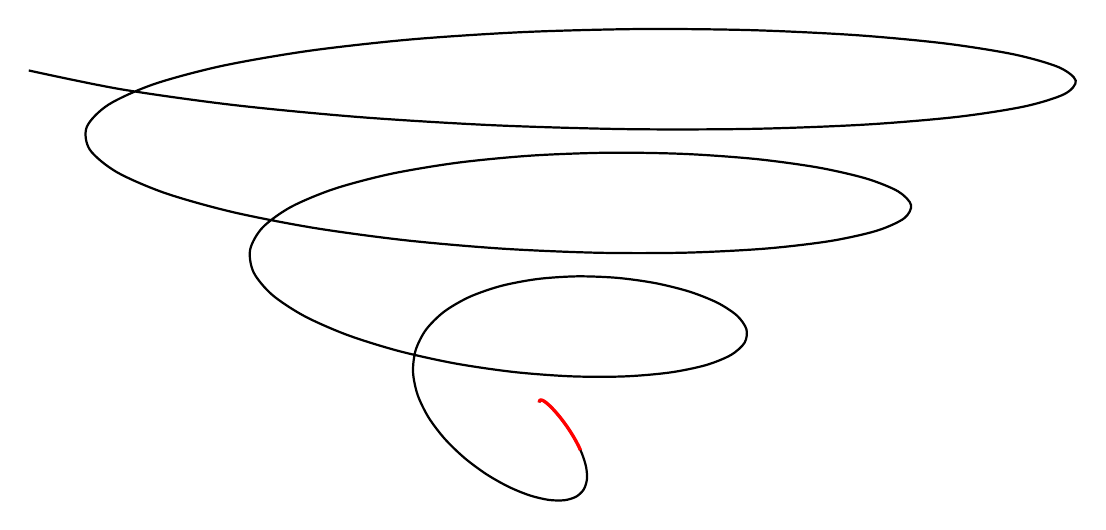
\begin{tikzpicture}
\draw[thick] plot[domain=0:23, smooth, samples=100]({sin( \x r)*\x/3},{cos(\x r)+\x/4});
\draw[very thick, red] plot[domain=0:1.57, smooth, samples=100]({sin( \x r)*\x/3},{cos(\x r)+\x/4});
\end{tikzpicture}
\end{center}
Due to the restricted domain, our actual curve is only one-quarter of a ``turn" of this spiral, indicated in red above.

The parameter $z$ is a measure of height, and it is also a radian measure as the spiral turns.
\end{solution}
%%%%%%%%%%%%%%%%%%


\begin{question}
Reparametrize the function $\vr(t)=(\tfrac12 t^2 , \tfrac13 t^3)$ in terms of arclength from $t=-1$.
\end{question}
\begin{hint}
Remember $\sqrt{x^2}=|x|$. You will need to consider cases for this one.
\end{hint}
\begin{answer}
$\vR(s)=\begin{cases}
\Big(\frac12\left[ (2\sqrt2-3s)^{2/3}-1)\right],-\frac13\left[(2\sqrt2-3s)^{2/3}-1\right]^{3/2}\Big)&\text{ when }s\le \frac13(2\sqrt2-1)\\
\Big(\frac12\left[(3s+2-2\sqrt2)^{2/3}-1 \right],\frac13\left[(3s+2-2\sqrt2)^{2/3}-1\right]^{3/2}\Big)&\text{ when }s>\frac13(2\sqrt2-1)
\end{cases}
$
\end{answer}
\begin{solution}
\begin{align*}
\vr(t)&=(\tfrac12 t^2 , \tfrac13 t^3)\\
\vr'(t)&=(t,t^2)\\
|\vr'(t)|&=\sqrt{t^2+t^4}=|t|\sqrt{1+t^2}\\
s(t)&=\int_{-1}^t|x|\sqrt{1+x^2}\dee{x}=\begin{cases}
\int_{-1}^t -x\sqrt{1+x^2}\dee{x} & \text{when } t \le 0\\
\int_{-1}^0 -x\sqrt{1+x^2}\dee{x} +\int_{0}^t x\sqrt{1+x^2}\dee{x} & \text{when } t > 0\\
\end{cases}
\intertext{Let $u=1+x^2$, $\frac12\dee{u}=x\dee{x}$}
&=\begin{cases}
-\int_{2}^{1+t^2} \frac{1}{2}\sqrt{u}\dee{u} & \text{when } t \le 0\\
-\int_{2}^1 \frac12\sqrt{u}\dee{u}+ \int_{1}^{1+t^2} \frac12\sqrt{u}\dee{u} & \text{when } t > 0\\
\end{cases}
\\&=\begin{cases}
 -\frac{1}{3}u^{3/2}|_{2}^{1+t^2} & \text{when } t \le 0\\
-\frac{1}{3}u^{3/2}|_{2}^{1}+  \frac13u^{3/2}|_{1}^{1+t^2} & \text{when } t > 0\\
\end{cases}
\\&=\begin{cases}
 \frac{2^{3/2}}{3}-\frac{1}{3}(1+t^2)^{3/2} & \text{when } t \le 0\\
-\frac23+\frac{2^{3/2}}{3}+\frac13(1+t^2)^{3/2} & \text{when } t > 0\\
\end{cases}
\intertext{Solving for $t$ in terms of $s$:}
1+t^2&=\begin{cases}(2\sqrt2-3s)^{2/3} &\text{when } t \le 0\\
(3s+2-2\sqrt{2})^{2/3} &\text{when }t>0\end{cases}\\
t^2&=\begin{cases}(2\sqrt2-3s)^{2/3}-1 &\text{when } t \le 0\\
(3s+2-2\sqrt{2})^{2/3}-1 &\text{when }t>0
\end{cases}
\intertext{Remembering that $\sqrt{t^2}=|t|$:}
t&=\begin{cases}-\sqrt{(2\sqrt2-3s)^{2/3}-1} &\text{when } t \le 0\\
\sqrt{(3s+2-2\sqrt{2})^{2/3}-1} &\text{when }t>0
\end{cases}
\intertext{Noting that $t=0$ when $s=\tfrac{1}{3}(2\sqrt2-1)$, we find our reparametrization of $(\tfrac12t^2,\tfrac13t^3)$.}
\vR(s)&=\begin{cases}
\Big(\frac12\left[ (2\sqrt2-3s)^{2/3}-1)\right],-\frac13\left[(2\sqrt2-3s)^{2/3}-1\right]^{3/2}\Big)&\text{ when }s\le \frac13(2\sqrt2-1)\\
\Big(\frac12\left[(3s+2-2\sqrt2)^{2/3}-1 \right],\frac13\left[(3s+2-2\sqrt2)^{2/3}-1\right]^{3/2}\Big)&\text{ when }s>\frac13(2\sqrt2-1)
\end{cases}
\end{align*}
Remark: after a computation with this much detail, it's nice to find a few points to check, to verify that our answer is reasonable. For instance, when $s=0$, $t$ should be $-1$, and vice-versa. Also, we found that $t=0$ corresponds to $s=\frac13(2\sqrt2-1)$. So, we should be able to verify that $\vr(0)=\vR\left(\frac13(2\sqrt2-1)\right)$ and $\vr(-1)=\vR(0)$.
\end{solution}
%%%%%%%%%%%%%%%%%%

%%%%%%%%%%%%%%%%%%
